\documentclass[../besoin_user.tex]{subfiles}
\begin{document}
\section{Connexion}
\begin{figure}[h]
    \centering
    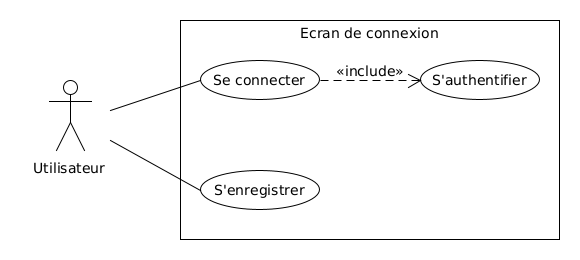
\includegraphics[scale=0.6]{img_fonctionnel/use_case_user_connexion.png}
    \label{fig:user_connexion}
    \caption{Connexion}
\end{figure}
  Lorsque le jeu est lancé, une fenêtre de connexion s'affiche, offrant à l'utilisateur la possibilité de se connecter à son compte. 
  Si l'utilisateur ne dispose pas encore d'un compte, il a la possibilité d'en créer un. 
  La creation d'un compte ne nécessite qu'un nom d'utilisateur valide, et un mot de passe. 
  Une fois l'authentification réussie, l'utilisateur est directement dirigé vers le menu principal du jeu, sans avoir à se connecter une fois de plus.
  \newpage
\end{document}